\chapter{Versuch 2: Passiver Zweipol}
\section{Einleitung}
Ziel dieses Versuch ist es von einem unbekannten Bauteil (BlackBox 3) zunächst
die Art der Bauteile zu bestimmen. Anschließend soll die Anordung der Bauteile
innerhalb der BlackBox bestimmt werden. Des weiteren wurde angegeben, dass es eine
Kombination aus 2 der folgenden Bauteile ist:
\begin{itemize}
    \item Widerstand R
    \item Kondensator C
    \item Spule L
\end{itemize}
Des Weiteren wird eine Methode zur Korrektur von Verzerrungen untersucht.

\section{Benötigte Geräte}

\begin{tabular}[h]{c|c}
	Backbox 3 & unbekannt \\
    \hline
    Funktionsgenerator & T3AFG80\\
    \hline
    Digital-Multimeter & Fluke TRUE RNS MULTIMETER\\
    \hline
    Oszilloskop & Keysight DSOX1102A
    \label{tab:Versuch 2: Geräte}
\end{tabular}

\section{Versuchsdurchführung}
Der Vorwiderstand aus Versuch 1 wurde verwendet. Der ausgemessene Wert hierführ
betrug R\textsubscript{v} = 4,583 k$\Omega$. Auch hier muss man wieder beachten, 
dass der Widerstand des Funktionsgenerators hier hinzuaddiert werden muss. 
Dieser beträgt R\textsubscript{i} = 50$\Omega$. Somit ergibt sich 
R\textsubscript{v*} = 4,633 k$\Omega$.

\subsection{Versuchsaufbau}

\begin{figure}[H]
	\centering
	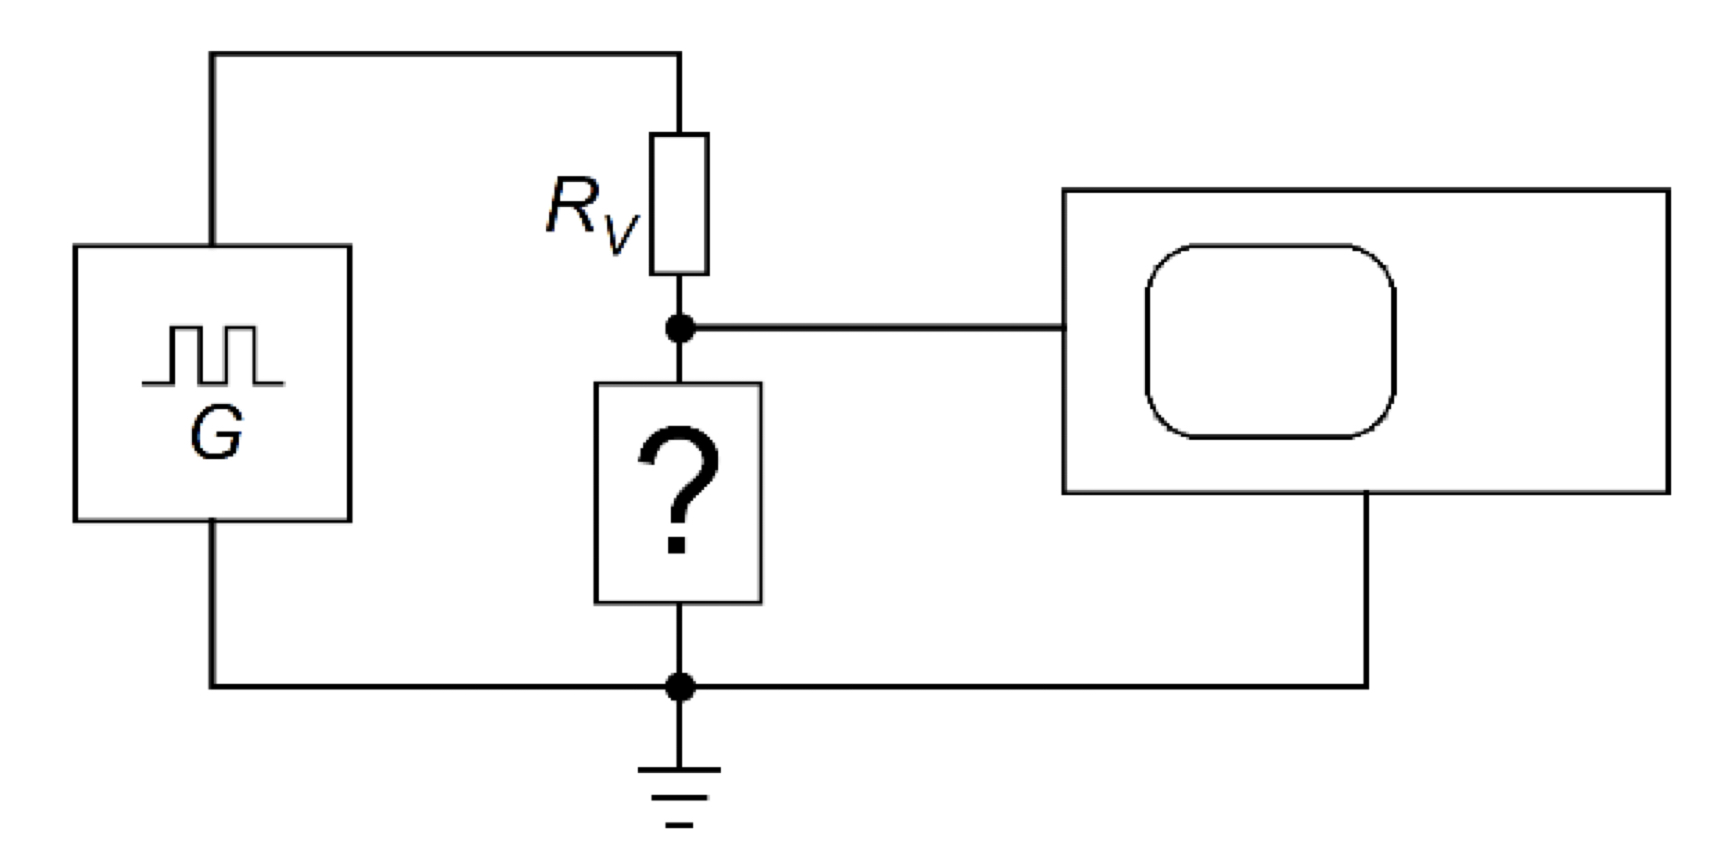
\includegraphics[height=7cm]{images/Versuch2/1_Schaltungsskizze.jpeg} 
	\caption{Schaltungsskizze}
	\label{fig: Schaltungsskizze}
\end{figure}

\subsection{Bauteile bestimmen}

\begin{figure}[H]
	\centering
	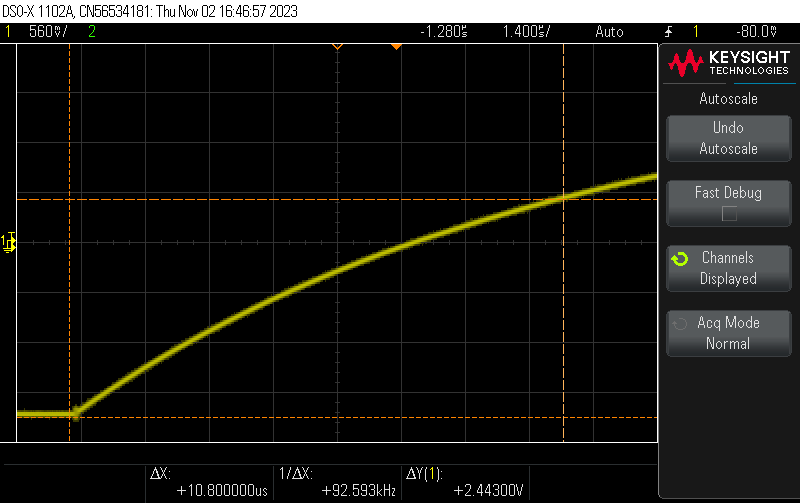
\includegraphics[height=7cm]{images/Versuch2/Zeitmessung_tau_10_8microsek.png} 
	\caption{Zeitmessung Ladekurve des Kondensators}
	\label{fig: Zeitmessung ladekurve des Kondensators}
\end{figure}

Durch das anschließen an das Oszilloskop wird ersichtlich, dass ein Bauteil ein 
Kondensator ist. Nun wird durch eine Messung mit dem Digital-Multimeter das zweite
Bauteil bestimmt. Dabei Messen wir einen Widerstand von 8,20k$\Omega$, sowie einen
Spannungsabfall von 1,588V. 

\begin{tabular}[h]{c|c|c|c}
    \textbf{Bauteil 1} & \textbf{Verschaltungsart} & \textbf{Bauteil 2} & \textbf{Widerstand der BlackBox}\\
    \hline
    Kondensator & parallel & Spule & 0 \\
    \hline
    Kondensator & in Reihe & Spule & $\infty$ \\
    \hline
    Kondensator & parallel & Wiederstand & =Widerstand \\
	\hline
	Kondensator & in Reihe & Widerstand & $\infty$ 
    \label{tab:Versuch 2: Bauteile bestimmen}
\end{tabular}

Da der Widerstand in der BlackBox nicht unendlich groß ist, kann es sich nicht um
eine Schltung in Reihe handeln. Da der Widerstand in der BlackBox nicht 0 ist, kann
es sich nicht um eine Parrallelschaltung mit einer Spule handeln. Somit muss es sich
um eine Parrallelschaltung mit einem Widerstand handeln. Dieser Widertsand ist (s.o.) 
$R\textsubscript{B}$ = 8,20k$\Omega$.
Mit dem Widerstand und der Frequenz kann nun die Kapazität des Kondensators berechnet.
Dafür verwendet man folgende Formeln:

\begin{equation}
	R\textsubscript{ges} = \frac{1}{\frac{1}{R\textsubscript{v*}} + 
	\frac{1}{R\textsubscript{B}}}
	\label{eq:Rges}
\end{equation}

mit Gleichung \ref*{eq:Rges} können wir nun R\textsubscript{ges} = 2,96k$\Omega$
berechnen.
$\tau$ = 10,8$\mu$s wurde am Oszilloskop abgelesen. Mit der Formel für die Kapazität
(Gleichung \ref*{eq:C})
\begin{equation}
	C = \frac{\tau}{R\textsubscript{ges}}
	\label{eq:C}
\end{equation}
können wir nun die C\textsubscript{B} = 3,648nF berechnen.


\section{Verzerrung des Signals}
\subsection{Schaltskizze}

\begin{figure}[H]
	\centering
	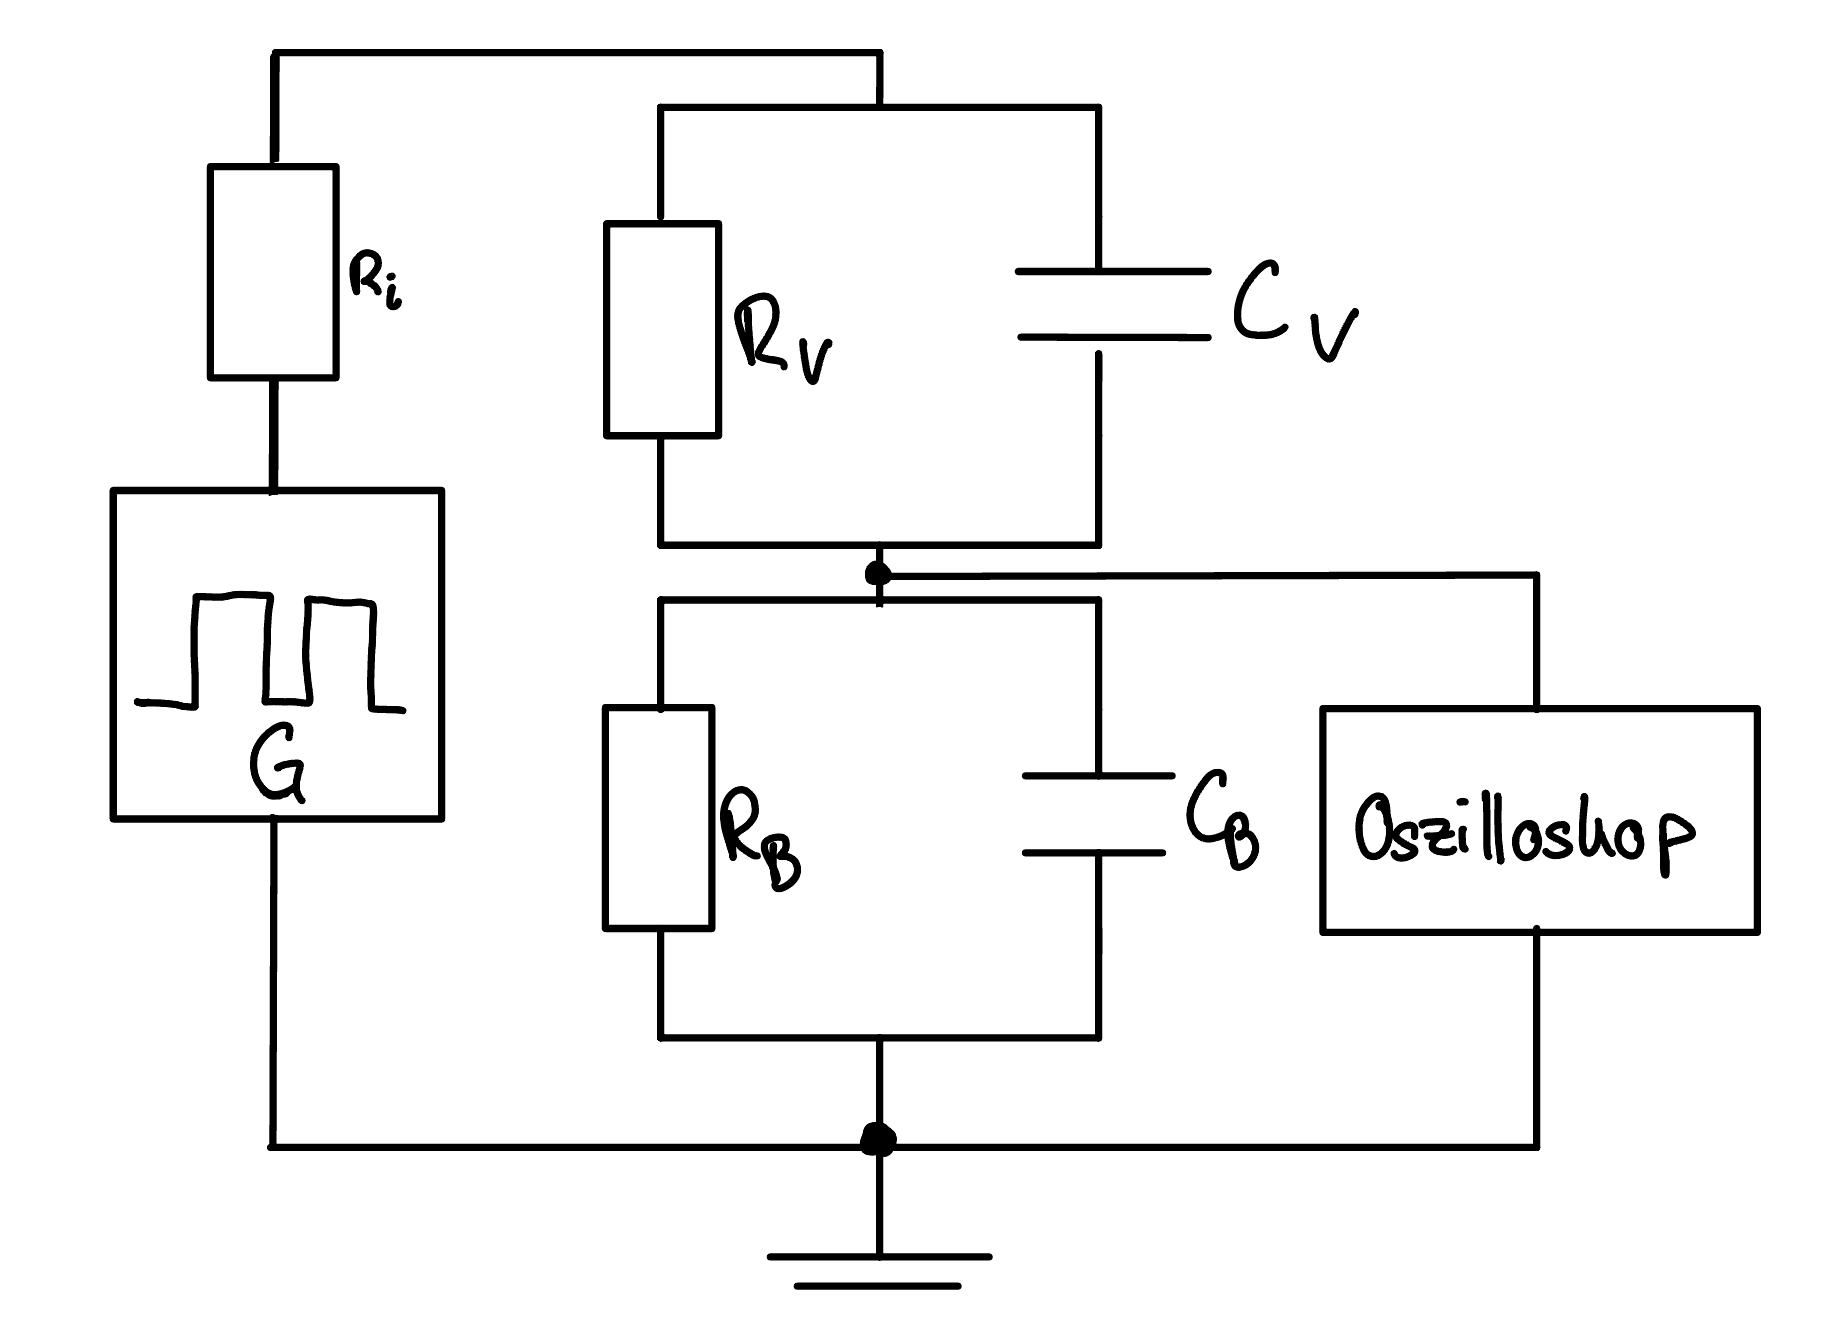
\includegraphics[height=7cm]{images/Versuch2/2_Schaltungsskizze.jpeg} 
	\caption{Schaltskizze}
	\label{fig: Schaltungsskizze}
\end{figure}

\subsection{Berchnung der Kapazität}

\begin{equation}
	\frac{R\textsubscript{V}}{R\textsubscript{B}} = \frac{C\textsubscript{V}}{C\textsubscript{B}}
	\label{eq:Cv}
\end{equation}

Durch Auflösung der Geleichung \ref*{eq:Cv} nach C\textsubscript{V}
erhalten wir: 

\begin{equation}
	C\textsubscript{V} = \frac{R\textsubscript{V}}{R\textsubscript{B}} \cdot C\textsubscript{B}
	\label{eq:Cv2}
\end{equation}

Durch das Hinzufügen eines weiteren Kondensators C\textsubscript{V} 
wird U\textsubscript{V} \textasciitilde U\textsubscript{0}
Mit den Werten auf 2.1 ergibt sich C\textsubscript{V} = 2,039nF.

\section{Zusatzfragen}

Das BNC Kabel addiert seine Kapazität parallel zur Schaltung.
Zur Vermeidung sollte mit Tastköpfen gearbeitet werden.




